\chapter*{Report}
\section*{Task 1}
\begin{table}[htpb]\centering
	\begin{tabular}{|l|l|l|l|}
		\hline
		Dataset     & Description                                                                                           & Format                                                                                                              & Parameters                                                                             \\ \hline
		GNSS        & \begin{tabular}[c]{@{}l@{}}The position change \\ of the transducers \\ measured by GNSS\end{tabular} & \multicolumn{1}{c|}{\begin{tabular}[c]{@{}c@{}}{[}ymd,h:m:s,\\ deg,deg,deg{]}\end{tabular}} & \begin{tabular}[c]{@{}l@{}}Date-Time-Lon-\\ Lat-Height\end{tabular}                    \\ \hline
		pxp-ini     & \begin{tabular}[c]{@{}l@{}}The coordiates of \\ the 4 transponders\end{tabular}                       & {[}deg:deg:m{]}                                                                                                     & \begin{tabular}[c]{@{}l@{}}Latitude-\\ Lontitude-\\ Depth\end{tabular}                 \\ \hline
		Sound Speed & \begin{tabular}[c]{@{}l@{}}The Depth-Sound \\ speed Modell in \\ Hawaii\end{tabular}                  & {[}m,m/s,deg-C,\%{]}                                                                                                & \begin{tabular}[c]{@{}l@{}}Depth,\\ SoundSpeed,\\ Temperature,\\ Salinity\end{tabular} \\ \hline
	\end{tabular}
\end{table}
The final results should be the location of the transponders or the location change of the transponders. \\\\
There is a offset between WG and transducer and another between the GNSS antenner and WG. So, the GNSS position needs to be corrected to get the true values. The latitude and lontitude will at first transformed into E and N, then the rotate and vertikal offset can be adjusted. After that the corrected E and N are transformed back to Lat and Lon. The GNSS position of the transducers and the sound travel time can present it.
\clearpage
\section*{Task 2 \& Task 3}
There is Outliers in the GNSS data, it needs to be filted out, than the trajectory kan be plotted. The red points are the 4 transponders.
\begin{figure}[htpb]\centering
	\subfigure[trajectory with out filting outliers]{
		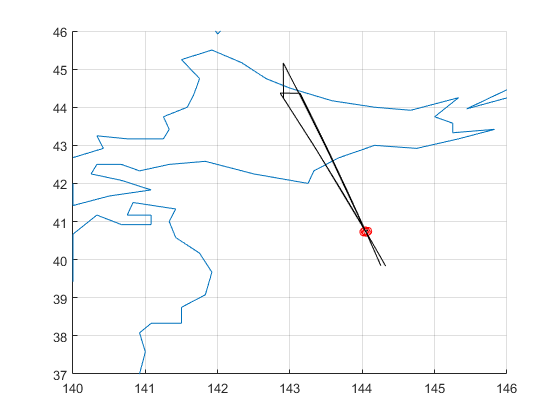
\includegraphics[width=0.6\textwidth]{task2_0.png}}
	\subfigure[trajectory]{
		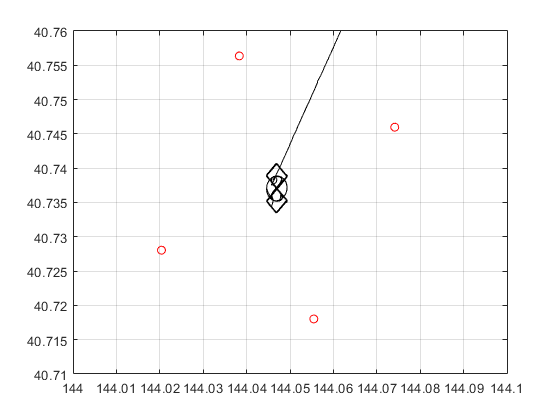
\includegraphics[width=0.6\textwidth]{task2_1.png}}
\end{figure}
\clearpage
\section*{Task 4}
The funciton rat-trace-chadwell calculates the one way travel time from a source to the receiver using a existed depth-speed Modell. The ThetaCheck parameter is here set to $35^{\circ}$.\\\\
The geodetic range are set to 0 but this parameter is somehow not used in the function.
\begin{figure}[htpb]\centering
	\subfigure[One way time]{
		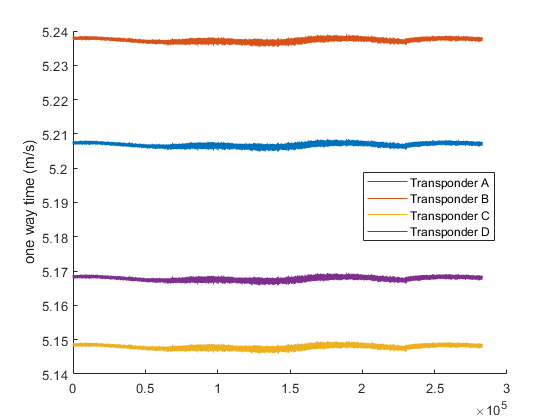
\includegraphics[width=0.9\textwidth]{task4.png}}
\end{figure}
\clearpage
\section*{Task 5}
There are several methods to calculate the one way time, which are chadwell, hovem, vnicent and julian. This funcTion will calculate the oneway time, eigen ray between receiver and source using one of those methods iteratively. 